% Provenance (never printed): see sources/outline_sources.md (Year 1: continental
% rifting and break-up; passive-margin structure; fast and slow ridges; the depth--age
% law of the ocean floor; transform faults). Curve from figdata/bachelor-1/depth_age.py;
% exercise and problem values in the Book 3 scratch calculator calc/ch13.py; the
% coordinates of the margin schematic from calc/fig13_margin.py.
\chapter{दरारें, कटक और निष्क्रिय किनारे}\label{ch:b1:rifts-ridges-margins}

सितंबर 2005 में इथियोपिया के उत्तर-पूर्व में अफ़ार मरुस्थल की ज़मीन खुल गई। तीन सप्ताह के भीतर लगभग \qty{60}{km} लंबे दरार-खंड का एक भाग \qty{8}{m} तक चौड़ा हो गया, और लगभग \qty{2.5}{km^3} मैग्मा नीचे से दरार में उठ आया। वहाँ की प्लेटें लगभग \qty{18}{mm} प्रति वर्ष पर अलग होती हैं: उस संकट ने कुछ सप्ताहों में लगभग चार सदियों का खिंचाव मुक्त कर दिया। अफ़ार एक टूटता हुआ महाद्वीप है; कुछ सौ किलोमीटर उत्तर में लाल सागर एक युवा महासागर है जिसका तल पहले से अटलांटिक के तल की तरह बना है, और दक्षिण अटलांटिक भी खुलने से पहले ऐसी ही एक दरार था, लगभग 120 मिलियन वर्ष पहले। यह अध्याय एक महासागर के जन्म का अनुसरण करता है: एक महाद्वीप का खिंचाव, उसका टूटना, पीछे छूटे दो निष्क्रिय किनारे, वह कटक जो महासागर-तल बनाता है, और ठंडे होते उस तल का धीमा धँसना।
% ledger: wright:afar, morvel:ar-nb (18.5 mm/yr at 12.3 N, 40.6 E, computed with euler_velocities.py), heine:fit

\begin{recall}
प्लेटें \omterm{def:b1:layered-earth:layers}{प्रावार} की ऊपरी \omterm{def:b1:heat-budget:boundary-layer}{ऊष्मीय सीमा-परत} हैं; महासागरों के नीचे एक ठंडा होता अर्ध-अंतरिक्ष उन्हें वर्णित करता है, और उनकी समतापीय रेखाएँ आयु के वर्गमूल के अनुपात में गहरी होती हैं (\cref{ch:b1:heat-budget})। समस्थैतिक साम्य में चट्टान के स्तंभ एक \omterm{def:b1:isostasy-gravity:isostasy}{प्रतिपूर्ति गहराई} के ऊपर प्रति एकाई क्षेत्रफल समान द्रव्यमान रखते हैं (\cref{ch:b1:isostasy-gravity})। प्लेटें यूलर ध्रुवों के परितः घूमती हैं, कटक चुंबकीय विसंगतियों से पढ़ी दरों से फैलते हैं, और रूपांतर ध्रुव के परितः लघुवृत्तों पर पड़ते हैं (\cref{ch:b1:plate-kinematics})। एक भ्रंश का \omterm{def:b1:cross-sections:throw}{विस्थापन} और \omterm{def:b1:cross-sections:throw}{क्षैतिज विस्थापन} \cref{ch:b1:cross-sections} में परिभाषित किए गए थे; एक सामान्य भ्रंश एक झुका हुआ भ्रंश है जिसका ऊपरी खंड नीचे खिसका है (पुस्तक 2, कक्षा 11)।
\end{recall}

\section{महाद्वीपीय दरार}

एक महाद्वीप जो अपने किनारों पर बलों से खिंचता है, समान रूप से पतला नहीं होता। उसकी भंगुर ऊपरी \omterm{def:b1:layered-earth:layers}{भूपर्पटी} सामान्य भ्रंशों के साथ टूटती है, और उनके बीच के खंड धँसते और झुकते हैं; नीचे, गरम निचली \omterm{def:b1:layered-earth:layers}{भूपर्पटी} और \omterm{def:b1:layered-earth:layers}{प्रावार} बहते हैं।

\begin{definition}[महाद्वीपीय दरार, ग्राबेन, अर्ध-ग्राबेन]\label{def:b1:rifts-ridges-margins:rift}
एक \emph{महाद्वीपीय दरार}\index{महाद्वीपीय दरार} एक लंबा, संकरा क्षेत्र है जहाँ एक महाद्वीप खिंच रहा है: सामान्य भ्रंशों से घिरा एक अवनमन, जिसमें भूकंप और प्रायः ज्वालामुखी होते हैं। एक \emph{ग्राबेन}\index{ग्राबेन} दो सामान्य भ्रंशों के बीच गिरा एक खंड है, जो एक-दूसरे की ओर झुकते हैं। एक \emph{अर्ध-ग्राबेन}\index{अर्ध-ग्राबेन} एक खंड है जो केवल एक ओर के एक प्रमुख सामान्य भ्रंश, सीमा-भ्रंश, के विरुद्ध गिरा और झुका हुआ है।
\end{definition}

अधिकांश दरार-द्रोणियाँ अर्ध-ग्राबेनों की शृंखलाएँ हैं। उनके सीमा-भ्रंश \omterm{def:b1:cross-sections:throw}{विस्थापन} को रिले-ढलानों के ज़रिए एक-दूसरे को सौंप देते हैं, और सीमा-भ्रंश की दिशा, एक खंड से अगले में, अक्सर बदलती रहती है। हर सीमा-भ्रंश की लटकती दीवार उसकी ओर नीचे झुकती है, और द्रोणी वहीं सबसे तेज़ भरती है: सबसे मोटा अवसाद भ्रंश से सटकर जमा होता है, जबकि पादभित्ति दरार-कंधे में ऊपर उठ जाती है।

किसी भ्रंश द्वारा वहन किया गया क्षैतिज खिंचाव उसका \omterm{def:b1:cross-sections:throw}{क्षैतिज विस्थापन} है। $h$ \omterm{def:b1:cross-sections:throw}{विस्थापन} और $\delta$ \omterm{def:b1:geological-maps:attitude}{नति} वाले एक समतल सामान्य भ्रंश का \omterm{def:b1:cross-sections:throw}{क्षैतिज विस्थापन} $h/\tan\delta$ है (\cref{ch:b1:cross-sections}); एक दरार-परिच्छेद में भ्रंशों के क्षैतिज विस्थापनों को जोड़ने से भंगुर \omterm{def:b1:layered-earth:layers}{भूपर्पटी} का विस्तार मिलता है। पूरा \omterm{def:b1:layered-earth:lithosphere}{स्थलमंडल} खिंचने पर कैसे पतला होता है, और फिर क्यों धँसता है, यह पुस्तक 4 में परिमाणित है; यहाँ भ्रंशों को मापा जाता है, और उनके योग की तुलना प्लेटों की गति से की जाती है।

\begin{omfigure}
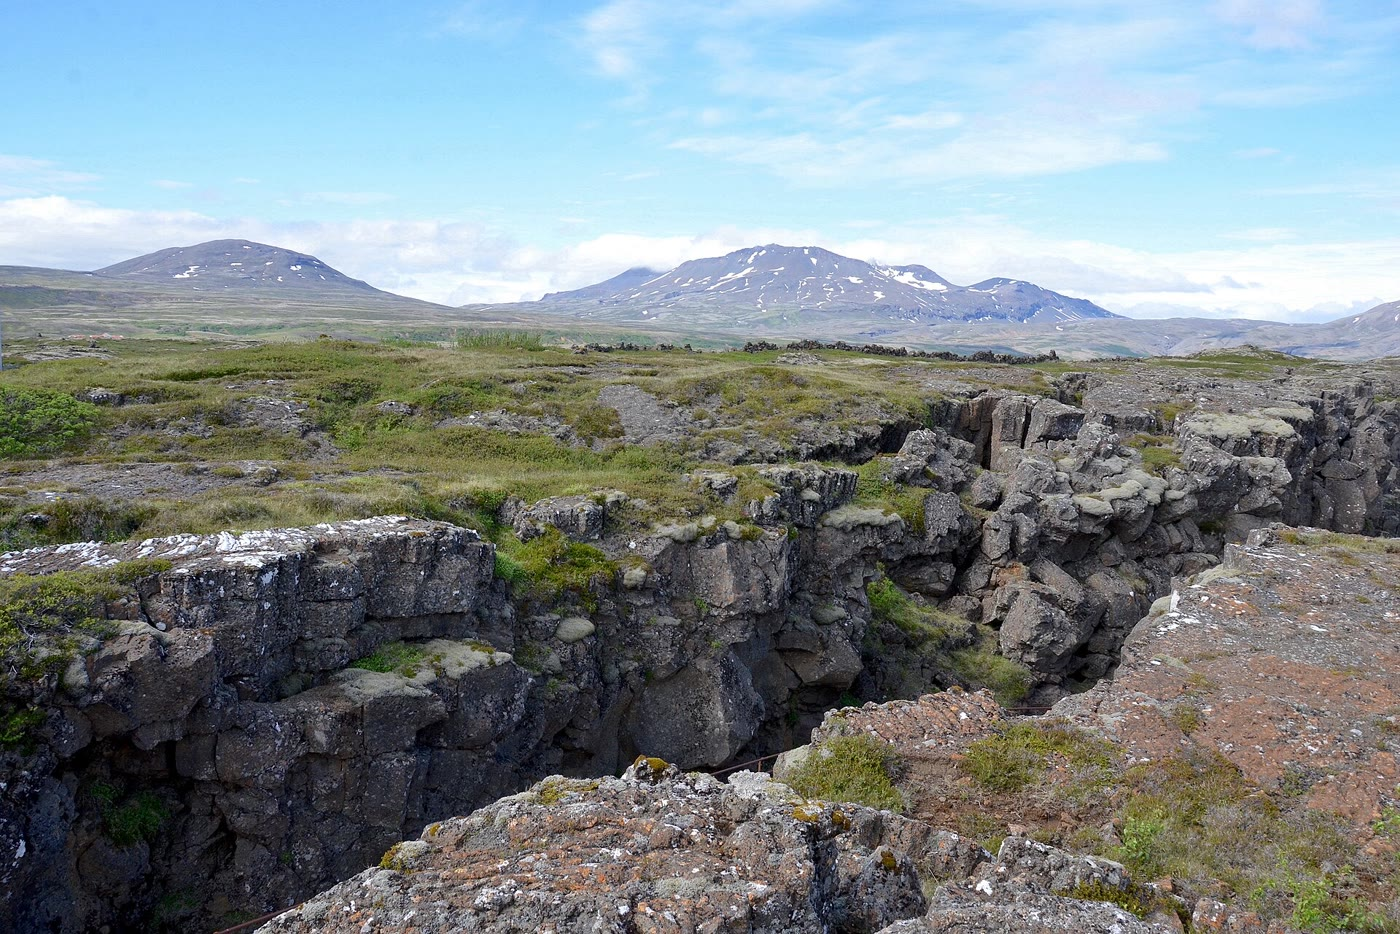
\includegraphics[width=0.8\linewidth]{images/book3/b1-thingvellir-fissure.jpg}

\par\smallskip{\small Þingvellir दरार-घाटी के लावा-तल में एक खुली दरार, दक्षिण-पश्चिम आइसलैंड में, जहाँ मध्य-अटलांटिक कटक समुद्र से ज़मीन पर आता है। घाटी के तल के बेसाल्ट प्रवाह दरार के समांतर खुली दरारों से कटे हैं। फ़ोटो: Olga Ernst,
CC~BY-SA~4.0 (Wikimedia Commons)।}
\label{fig:b1:rifts-ridges-margins:thingvellir}
\end{omfigure}
% ledger: commons:thingvellir

\subsection*{ज्वालामुखी और मैग्मा-विरल दरारें}

दरारें इस बात में भिन्न हैं कि उन्हें कितना मैग्मा मिलता है। एक \emph{मैग्मा-विरल} दरार में खिंचाव भ्रंशों द्वारा वहन होता है, और खंडों के खिसकने पर \omterm{def:b1:layered-earth:layers}{भूपर्पटी} पतली होती है। एक ज्वालामुखी दरार में मैग्मा कमान संभाल लेता है: अक्ष के साथ \omterm{def:b1:layered-earth:layers}{भूपर्पटी} में डाइक घुसते हैं, जिनमें से हर एक दरार को अपनी मोटाई भर खोलता है, और लावा सतह को भर देता है। पूर्वी अफ़्रीकी दरार दोनों दिखाती है, साथ-साथ: उसकी पूर्वी शाखा तीव्र रूप से ज्वालामुखी-सक्रिय है, जबकि पश्चिमी शाखा उतनी नहीं है और गहरे अवसादी द्रोणियाँ रखती है, जो तांगानिका झील जैसी झीलों से भरी हैं और भ्रंशों से घिरी हैं।
% ledger: roberts:ear

दोनों शाखाएँ लगभग 25 मिलियन वर्ष पहले बननी शुरू हुईं, और दरार अफ़्रीकी प्लेट को पश्चिम में एक नूबियन प्लेट और पूर्व में एक सोमाली प्लेट में बाँटती है। अफ़ार \omterm{def:b1:plate-kinematics:triple-junction}{त्रि-संधि} से वह दक्षिण की ओर चलती है, पुराने, मोटे और ठंडे तंज़ानिया क्रेटन के चारों ओर दो शाखाओं में। इसकी गति धीमी है: सोमालिया और नूबिया के प्लेट सदिशों से परिकलित, जिनमें से हर एक अंटार्कटिक प्लेट के सापेक्ष मापा गया है, सोमालिया नूबिया से \qty{6.0}{mm.yr^{-1}} पर \ang{105} की ओर, मध्य इथियोपिया (\ang{8.5}\,N, \ang{39.5}\,E) में, दूर जाता है, और भूमध्य रेखा पर \qty{5.1}{mm.yr^{-1}} पर। दरार के कई भूकंप सामान्य भ्रंशन दिखाते हैं।
% ledger: roberts:ear, morvel:sm-an, morvel:nb-an (SM-NB from SM-AN minus NB-AN, computed with figdata/bachelor-1/euler_velocities.py)

अफ़ार में, उत्तरी सिरे पर, दरार लाल सागर और अदन की खाड़ी से मिलती है। इथियोपियाई बाढ़-बेसाल्ट का अधिकांश भाग वहाँ लगभग 30 मिलियन वर्ष पहले, एक मिलियन वर्ष या उससे कम में, फूटा, और तब से मैग्मा लगातार आता रहा है: सतह पर लावा-प्रवाह, \omterm{def:b1:layered-earth:layers}{भूपर्पटी} में अंतर्वेधन और उसके नीचे नई सामग्री का जुड़ना, इतना कि अंतर्विष्ट \omterm{def:b1:layered-earth:layers}{भूपर्पटी} ने दरार की प्रारंभिक अवस्थाओं में अपनी मोटाई बनाए रखी। 2005 का संकट दिखाता है कि ऐसी दरार कैसे खुलती है: एकसमान रूप से नहीं, बल्कि प्रकरणों में, हर एक एक डाइक जो मीटरों चौड़ा है और दिनों या सप्ताहों में अंतर्विष्ट होता है। चूँकि वहाँ प्लेटें लगभग \qty{18}{mm.yr^{-1}} पर अलग होती हैं, 2005 के \qty{8}{m} डाइक ने लगभग 440 वर्षों के खिंचाव को समाहित किया।
% ledger: hofmann:traps, bastow:afar, wright:afar, morvel:ar-nb (rate computed with euler_velocities.py)

\section{टूटना और निष्क्रिय किनारे}

यदि खिंचाव जारी रहता है, तो महाद्वीपीय \omterm{def:b1:layered-earth:layers}{भूपर्पटी} शून्य तक पतली हो जाती है, दरार के नीचे \omterm{def:b1:layered-earth:layers}{प्रावार} उठता है और उठते हुए पिघलता है, और महाद्वीप के दो अर्ध-भागों के बीच पहली \omterm{def:b1:rifts-ridges-margins:oceanic-crust}{महासागरीय भूपर्पटी} बनती है। वह क्षण \emph{टूटना} है। उसके बाद प्लेटें एक नए महासागर के बीच एक कटक पर अलग होती हैं, और महाद्वीप के दोनों किनारे, कटक से दूर ले जाए जाकर, प्लेट-सीमाएँ नहीं रहते।

\begin{definition}[निष्क्रिय किनारा, महासागर–महाद्वीप संक्रमण, टूटन-असंगति]\label{def:b1:rifts-ridges-margins:passive-margin}
एक \emph{निष्क्रिय किनारा}\index{निष्क्रिय किनारा} एक महाद्वीप का वह किनारा है जो दरार से बना और अब प्लेट-सीमा नहीं है: महाद्वीप और सटा महासागर-तल एक ही प्लेट के हैं। \emph{महासागर–महाद्वीप संक्रमण}\index{महासागर–महाद्वीप संक्रमण} किनारे का वह क्षेत्र है, किलोमीटर से दसियों किलोमीटर चौड़ा, जो पतली महाद्वीपीय \omterm{def:b1:layered-earth:layers}{भूपर्पटी} और सामान्य \omterm{def:b1:rifts-ridges-margins:oceanic-crust}{महासागरीय भूपर्पटी} के बीच है। \emph{टूटन-असंगति}\index{टूटन-असंगति} वह \omterm{def:b1:cross-sections:unconformity}{असंगति} है जो दरार-द्रोणियों में जमा अवसादों को, उनके खंडों के साथ झुके हुए, टूटने के बाद किनारे पर बिछे अविक्षुब्ध अवसादों से अलग करती है।
\end{definition}

निष्क्रिय किनारे अटलांटिक के अधिकांश, आर्कटिक महासागर और पश्चिमी हिंद महासागर को रेखांकित करते हैं, और अफ़्रीका, ऑस्ट्रेलिया, ग्रीनलैंड और भारत के लगभग सभी तट। उत्तर अमेरिका का पूर्वी किनारा और अफ़्रीका का उत्तर-पश्चिमी किनारा एक ही दरार के दो पक्ष थे: वे \emph{संयुग्मी} किनारे हैं। उनकी परिच्छेदिका ज़मीन के निकट महासागर-तल का परिचित क्रम है: महाद्वीपीय शेल्फ, ढलान, उभार और अतल मैदान। शेल्फ और ढलान के नीचे पतली महाद्वीपीय \omterm{def:b1:layered-earth:layers}{भूपर्पटी} है, सामान्य भ्रंशों से कटी जो महासागर की ओर झुकते हैं, उनके घूमे हुए खंड अवसादों के नीचे दबे हुए।

\begin{omfigure}
\begin{tikzpicture}[x=0.95cm, y=0.9cm, font=\scriptsize]
% (a) continental rift: half-grabens on east-dipping faults; coordinates from calc/fig13_margin.py
\begin{scope}
\fill[green!25!gray!45] (0,-2) -- (3,-2) -- (6,-1.75) -- (9,-2) -- (12,-2) -- (12,-2.5) -- (0,-2.5) -- cycle;
\fill[orange!22] (0,0) -- (3.5,0) -- (3.931,-0.8) -- (4.75,-0.25) -- (5.05,-0.7) -- (6,-0.2) -- (6.223,-0.55) -- (7.25,-0.15) -- (7.402,-0.4) -- (8.6,0) -- (12,0) -- (12,-2) -- (9,-2) -- (6,-1.75) -- (3,-2) -- (0,-2) -- cycle;
\fill[yellow!45] (3.565,-0.12) -- (3.931,-0.8) -- (4.75,-0.25) -- (4.75,-0.12) -- cycle;
\fill[yellow!45] (4.75,-0.12) -- (4.75,-0.25) -- (5.05,-0.7) -- (6,-0.2) -- (6,-0.12) -- cycle;
\fill[yellow!45] (6,-0.12) -- (6,-0.2) -- (6.223,-0.55) -- (7.25,-0.15) -- (7.25,-0.12) -- cycle;
\fill[yellow!45] (7.25,-0.12) -- (7.25,-0.15) -- (7.402,-0.4) -- (8.241,-0.12) -- cycle;
\draw (0,0) -- (3.5,0) -- (3.931,-0.8) -- (4.75,-0.25) -- (5.05,-0.7) -- (6,-0.2) -- (6.223,-0.55) -- (7.25,-0.15) -- (7.402,-0.4) -- (8.6,0) -- (12,0);
\draw[contact] (0,-2) -- (3,-2) -- (6,-1.75) -- (9,-2) -- (12,-2);
\draw[fault] (3.5,0) -- (4.2,-1.3);
\draw[fault] (4.75,-0.25) -- (5.45,-1.3);
\draw[fault] (6,-0.2) -- (6.7,-1.3);
\draw[fault] (7.25,-0.15) -- (7.95,-1.3);
\node[anchor=west, font=\small\bfseries] at (0,0.75) {(क) महाद्वीपीय दरार};
\node[anchor=south] at (2.2,0) {दरार-कंधा};
\node[anchor=south, align=center] at (6.3,0) {अवसाद से भरे अर्ध-ग्राबेन};
\draw[-{Stealth[length=3pt]}] (2.6,-0.75) node[anchor=east] {सीमा-भ्रंश} -- (3.75,-0.5);
\node at (9.8,-1.0) {महाद्वीपीय भूपर्पटी};
\node at (10.3,-2.25) {प्रावार};
\node at (6,-2.18) {दरार के नीचे उठा मोहो};
\end{scope}
% (b) break-up: conjugate halves, the first oceanic crust between them
\begin{scope}[yshift=-3.6cm]
\fill[omSea!35] (2.8,0) -- (9.2,0) -- (9.2,-1.3) -- (2.8,-1.3) -- cycle;
\fill[green!25!gray!45] (0,-2) -- (2.5,-2) -- (5.5,-1.3) -- (6.5,-1.3) -- (9.5,-2) -- (12,-2) -- (12,-2.5) -- (0,-2.5) -- cycle;
\fill[orange!22] (0,0) -- (2.8,0) -- (3.146,-0.75) -- (3.8,-0.3) -- (4.13,-0.85) -- (4.7,-0.45) -- (5.053,-0.95) -- (5.5,-1) -- (5.5,-1.3) -- (2.5,-2) -- (0,-2) -- cycle;
\fill[orange!22] (12,0) -- (9.2,0) -- (8.854,-0.75) -- (8.2,-0.3) -- (7.87,-0.85) -- (7.3,-0.45) -- (6.947,-0.95) -- (6.5,-1) -- (6.5,-1.3) -- (9.5,-2) -- (12,-2) -- cycle;
\fill[lith basalt] (5.5,-1) -- (6.5,-1) -- (6.5,-1.3) -- (5.5,-1.3) -- cycle;
\draw (0,0) -- (2.8,0) -- (3.146,-0.75) -- (3.8,-0.3) -- (4.13,-0.85) -- (4.7,-0.45) -- (5.053,-0.95) -- (5.5,-1) -- (6.5,-1) -- (6.947,-0.95) -- (7.3,-0.45) -- (7.87,-0.85) -- (8.2,-0.3) -- (8.854,-0.75) -- (9.2,0) -- (12,0);
\draw[contact] (0,-2) -- (2.5,-2) -- (5.5,-1.3) -- (6.5,-1.3) -- (9.5,-2) -- (12,-2);
\draw[omSea!70!black] (2.8,0) -- (9.2,0);
\draw[fault] (2.8,0) -- (3.4,-1.3);
\draw[fault] (3.8,-0.3) -- (4.4,-1.3);
\draw[fault] (4.7,-0.45) -- (5.3,-1.3);
\draw[fault] (9.2,0) -- (8.6,-1.3);
\draw[fault] (8.2,-0.3) -- (7.6,-1.3);
\draw[fault] (7.3,-0.45) -- (6.7,-1.3);
\draw[omRidge, very thick, -{Stealth[length=3pt]}] (6,-2.3) -- (6,-1.45);
\node[anchor=west, font=\small\bfseries] at (0,0.75) {(ख) टूटना};
\node[anchor=south] at (6,0) {समुद्र दरार को भर देता है};
\node[anchor=west] at (6.15,-2.1) {प्रावार उठता और पिघलता है};
\node[anchor=south, fill=white, fill opacity=0.8, text opacity=1, inner sep=1pt, align=center] at (6,-0.85) {पहली महासागरीय\\भूपर्पटी};
\node at (1.4,-1.0) {झुके हुए खंड};
\node at (10.6,-1.0) {झुके हुए खंड};
\node at (1.4,-2.25) {प्रावार};
\end{scope}
% (c) one passive margin after drift
\begin{scope}[yshift=-7.4cm]
\fill[omSea!35] (1.2,0.3) -- (12,0.3) -- (12,-1.2) -- (8.2,-1.15) -- (6.4,-0.9) -- (4.6,0.1) -- cycle;
\fill[green!25!gray!45] (0,-2.3) -- (2,-2.3) -- (5.9,-1.8) -- (6.7,-2.1) -- (12,-2.1) -- (12,-2.7) -- (0,-2.7) -- cycle;
\fill[orange!22] (0,0.3) -- (1.2,0.3) -- (2.2,0) -- (3,-0.25) -- (3.259,-0.95) -- (4,-0.55) -- (4.286,-1.15) -- (4.9,-0.85) -- (5.233,-1.35) -- (5.9,-1.55) -- (5.9,-1.8) -- (2,-2.3) -- (0,-2.3) -- cycle;
\fill[pattern=crosshatch dots, pattern color=green!40!black] (5.9,-1.55) -- (6.4,-1.75) -- (6.7,-2.1) -- (5.9,-1.8) -- cycle;
\fill[lith basalt] (6.4,-1.75) -- (12,-1.75) -- (12,-2.1) -- (6.7,-2.1) -- cycle;
\fill[yellow!45] (3,-0.25) -- (3.259,-0.95) -- (4,-0.55) -- cycle;
\fill[yellow!45] (4,-0.55) -- (4.286,-1.15) -- (4.9,-0.85) -- cycle;
\fill[yellow!45] (4.9,-0.85) -- (5.233,-1.35) -- (5.9,-1.55) -- (5.9,-1.45) -- cycle;
\fill[yellow!15] (1.2,0.3) -- (4.6,0.1) -- (6.4,-0.9) -- (8.2,-1.15) -- (12,-1.2) -- (12,-1.75) -- (6.4,-1.75) -- (5.9,-1.55) -- (5.9,-1.45) -- (4.9,-0.85) -- (4,-0.55) -- (3,-0.25) -- (2.2,0) -- cycle;
\draw[black!45] (2.4,0.12) -- (4.8,-0.1) -- (6.6,-1.05) -- (8.4,-1.27) -- (12,-1.31);
\draw (1.2,0.3) -- (4.6,0.1) -- (6.4,-0.9) -- (8.2,-1.15) -- (12,-1.2);
\draw[omSea!70!black] (1.2,0.3) -- (12,0.3);
\draw[unconformity] (2.2,0) -- (3,-0.25) -- (4,-0.55) -- (4.9,-0.85) -- (5.9,-1.45);
\draw (3.259,-0.95) -- (4,-0.55) (4.286,-1.15) -- (4.9,-0.85) (5.233,-1.35) -- (5.9,-1.55) -- (6.4,-1.75) -- (12,-1.75);
\draw[contact] (0,-2.3) -- (2,-2.3) -- (5.9,-1.8) -- (6.7,-2.1) -- (12,-2.1);
\draw[fault] (3,-0.25) -- (3.5,-1.6);
\draw[fault] (4,-0.55) -- (4.5,-1.6);
\draw[fault] (4.9,-0.85) -- (5.4,-1.6);
\node[anchor=west, font=\small\bfseries] at (0,0.95) {(ग) निष्क्रिय किनारा};
\node[anchor=south] at (3.4,0.25) {शेल्फ};
\node[anchor=south west] at (5.6,-0.45) {ढलान};
\node[anchor=south] at (8.4,-1.12) {उभार};
\node[anchor=south] at (10.6,-1.17) {अतल मैदान};
\node[anchor=south] at (10.6,-0.1) {महासागर};
\node at (9.8,-1.53) {टूटन-पश्चात अवसाद};
\node[fill=white, fill opacity=0.8, text opacity=1, inner sep=1pt, align=center] (bu) at (1.0,-0.6) {टूटन-\\असंगति};
\draw[-{Stealth[length=3pt]}] (bu.east) -- (2.55,-0.16);
\node[fill=white, fill opacity=0.8, text opacity=1, inner sep=1pt, align=center] (sr) at (1.6,-1.35) {दरार-कालीन\\अवसाद};
\draw[-{Stealth[length=3pt]}] (sr.east) -- (3.45,-0.75);
\node at (1.3,-1.98) {महाद्वीपीय भूपर्पटी};
\draw[decorate, decoration={brace, amplitude=3pt, mirror}] (5.9,-2.17) -- (6.7,-2.17) node[midway, below=3pt, align=center] {महासागर–महाद्वीप\\संक्रमण};
\node[anchor=west, fill=white, fill opacity=0.85, text opacity=1, inner sep=1pt] at (8.6,-1.93) {महासागरीय भूपर्पटी};
\node at (3.6,-2.5) {प्रावार};
\end{scope}
\end{tikzpicture}

\par\smallskip{\small दरार से निष्क्रिय किनारे तक (चित्र, पैमाने पर नहीं; ऊँचाइयाँ बढ़ाई गई हैं)। (क) भंगुर ऊपरी \omterm{def:b1:layered-earth:layers}{भूपर्पटी} सामान्य भ्रंशों के साथ टूटती है; खंड अर्ध-ग्राबेनों में झुकते हैं जो अवसाद से भरते हैं, और पतली \omterm{def:b1:layered-earth:layers}{भूपर्पटी} के नीचे \omterm{def:b1:layered-earth:discontinuity}{मोहो} उठता है। (ख) टूटने पर महाद्वीपीय \omterm{def:b1:layered-earth:layers}{भूपर्पटी} आर-पार कट जाती है; समुद्र दरार को भर देता है और पहली \omterm{def:b1:rifts-ridges-margins:oceanic-crust}{महासागरीय भूपर्पटी} बनती है। (ग) दो किनारों में से एक, कटक से दूर ले जाया गया: उसके झुके हुए खंड और उनके अवसाद \omterm{def:b1:rifts-ridges-margins:passive-margin}{टूटन-असंगति} के नीचे पड़े हैं, शेल्फ, ढलान और उभार के टूटन-पश्चात अवसादों से दबे हुए।}
\label{fig:b1:rifts-ridges-margins:margin}
\end{omfigure}

\subsection*{दो प्रकार के किनारे}

किनारे अपनी दरार का चरित्र विरासत में पाते हैं। \emph{मैग्मा-विरल} किनारों पर, जैसे इबेरिया और न्यूफ़ाउंडलैंड के, भूकंप-परिच्छेद घूमे हुए खंड दिखाते हैं जिनकी परतें महाद्वीप की ओर झुकती हैं; कुछ स्थानों पर ऊँचा-नीचा संक्रमण \omterm{def:b1:layered-earth:layers}{प्रावार} की पेरिडोटाइट से बिछा है, जो समुद्र-तल तक लाई गई और समुद्र के पानी से सर्पेंटीनाइट में बदली गई। \emph{ज्वालामुखी} किनारों पर, जैसे मध्य-नॉर्वे, पूर्वी ग्रीनलैंड, नामीबियाई और ब्राज़ीली किनारों पर, संक्रमण बेसाल्ट से बना है: लावा प्रवाहों के ढेर जो महासागर की ओर झुकते हैं, भूकंप-परिच्छेदों के समुद्र की ओर झुके परावर्तक, और उनके नीचे एक निचली \omterm{def:b1:layered-earth:layers}{भूपर्पटी} जिसमें P तरंगें असामान्य रूप से तेज़ चलती हैं, टूटने पर \omterm{def:b1:layered-earth:layers}{भूपर्पटी} के नीचे जोड़ा गया मैग्मा। ज्वालामुखी किनारे टूटने के दौरान बहुत कम धँसते हैं।

\begin{inthefield}[महाद्वीप के किनारे का पता लगाना]
\omterm{def:b1:rifts-ridges-margins:passive-margin}{महासागर–महाद्वीप संक्रमण} किलोमीटरों पानी और अवसाद के नीचे है, और केवल भूभौतिकी से, आम तौर पर कई विधियों को एक साथ लगाकर, खोजा जाता है। भूकंपीय परावर्तन झुके हुए खंड, \omterm{def:b1:rifts-ridges-margins:passive-margin}{टूटन-असंगति} और, जहाँ संकेत पर्याप्त गहराई तक पहुँचता है, \omterm{def:b1:layered-earth:discontinuity}{मोहो} को दिखाता है। चौड़े-कोण का भूकंपीय अपवर्तन P तरंगों की चालें मापता है जो \omterm{def:b1:layered-earth:layers}{भूपर्पटी} से होकर जाती हैं, और महाद्वीपीय और \omterm{def:b1:rifts-ridges-margins:oceanic-crust}{महासागरीय भूपर्पटी} में ये भिन्न होती हैं। गुरुत्व आँकड़े, \omterm{def:b1:layered-earth:discontinuity}{मोहो} की गहराई के लिए व्युत्क्रमित, \omterm{def:b1:layered-earth:layers}{भूपर्पटी} की मोटाई देते हैं। महासागर-तल की चुंबकीय धारियाँ वहीं रुकती हैं जहाँ चुंबकीय रूप से शांत महाद्वीपीय \omterm{def:b1:layered-earth:layers}{भूपर्पटी} शुरू होती है।
\end{inthefield}

टूटने के बाद किनारा धँसता है। दरार के दौरान \omterm{def:b1:layered-earth:lithosphere}{स्थलमंडल} पतला और गरम हुआ था; कटक से दूर ले जाए जाने पर, वह ठंडा होता है और सिकुड़ता है, अपने बगल के महासागर-तल की तरह, और उसके ऊपर खुलने वाला स्थान टूटन-पश्चात अवसादों की पच्चर से भरता है, जिसका भार उसे और नीचे दबाता है। इस कहानी का शीतलन वाला भाग \cref{sec:b1:rifts-ridges-margins:depth-age} में कहा गया है; अवसादों का भार \cref{ch:b1:diagenesis-basins} का विषय है।

\section{तेज़ और धीमे कटक}

एक बार महासागर जन्म लेता है, वह अपने कटक पर बढ़ता है। कटक बहुत भिन्न दरों पर फैलते हैं: पिछले कुछ मिलियन वर्षों में मापी गई दरें लाल सागर के उत्तरी भाग में \qty{9.7}{mm.yr^{-1}} से पूर्वी प्रशांत उभार पर \qty{154.4}{mm.yr^{-1}} तक चलती हैं। उनका आकार उस दर पर निर्भर करता है।
% ledger: morvel:range

\begin{definition}[तेज़-, धीमे- और अति-धीमे-प्रसार कटक]\label{def:b1:rifts-ridges-margins:ridge-classes}
कटक को उसकी \omterm{def:b1:plate-kinematics:spreading-rate}{पूर्ण प्रसार-दर} से वर्गीकृत किया जाता है। एक \emph{अति-धीमा प्रसार कटक}\index{अति-धीमा प्रसार कटक} लगभग \qty{20}{mm.yr^{-1}} से कम पर खुलता है; एक \emph{धीमा प्रसार कटक}\index{धीमा प्रसार कटक} 20 से \qty{55}{mm.yr^{-1}} पर; एक मध्यवर्ती कटक 55 से \qty{75}{mm.yr^{-1}} पर; एक \emph{तेज़ प्रसार कटक}\index{तेज़ प्रसार कटक} लगभग \qty{75}{mm.yr^{-1}} से अधिक पर।
\end{definition}
% ledger: seton:rate-classes, dick:ultraslow

सीमाएँ परंपराएँ हैं और लेखकों के बीच भिन्न हैं। जो नहीं बदलता वह रूप का परिवर्तन है। एक धीमा कटक, जैसे मध्य-अटलांटिक कटक, में अंदर की ओर मुँह किए सामान्य भ्रंशों के बीच एक अक्षीय घाटी होती है: प्लेटों के बीच का अंतर उतनी तेज़ी से मैग्मा से नहीं भरता जितनी तेज़ी से वह खुलता है, और ठंडा \omterm{def:b1:layered-earth:lithosphere}{स्थलमंडल} टूट जाता है। एक तेज़ कटक, जैसे पूर्वी प्रशांत उभार, में कोई दरार-घाटी नहीं होती, बल्कि पिघलने के लेंस के ऊपर एक चिकना अक्षीय उभार होता है, जो बार-बार पर्याप्त भरा जाता है ताकि गति बनी रहे। दोनों ही स्थितियों में अक्ष लगभग \qty{2500}{m} गहरा है, और द्रोणियों का सबसे पुराना तल लगभग \qty{4}{km} और गहरा है (\cref{sec:b1:rifts-ridges-margins:depth-age})।
% ledger: parsons:plate-model (6400 - 2500 m)

अति-धीमे कटक दिखाते हैं कि मैग्मा सबसे कम होने पर क्या होता है: उनका ज्वालामुखीपन रुक-रुककर होता है, उनमें \omterm{def:b1:rifts-ridges-margins:transform}{रूपांतर भ्रंश} नहीं होते, और बड़े क्षेत्रों में \omterm{def:b1:layered-earth:layers}{प्रावार} स्वयं समुद्र-तल तक लाया जाता है। गाक्कल कटक, आर्कटिक महासागर के नीचे, सबसे धीमा, बिल्कुल विस्थापित नहीं है; उसके अक्ष के एक मध्य भाग के साथ, लगभग \qty{300}{km} लंबा, \omterm{def:b1:layered-earth:layers}{प्रावार} की पेरिडोटाइट अक्ष पर सीधे पड़ी है, पश्चिम में प्रचुर ज्वालामुखीपन और पूर्व में बड़े, दूर-दूर ज्वालामुखियों के बीच। विशेष रूप से धीमे और अति-धीमे कटकों पर, प्रसार का कुछ भाग लंबे, मंद रूप से झुके सामान्य भ्रंशों, विच्छेदों (डिटैचमेंट्स) से वहन होता है, जिनकी पादभित्ति अक्ष के नीचे से बाहर खींची जाती है: गैब्रो और पेरिडोटाइट लहरदार गुंबदों में समुद्र-तल तक पहुँचते हैं, \emph{महासागरीय कोर कॉम्प्लेक्स}। अटलांटिस मैसिफ़, लगभग \ang{30}\,N पर मध्य-अटलांटिक कटक के बगल में, एक ऐसा ही है: उसकी चोटी पर, कटक-अक्ष से लगभग \qty{15}{km} दूर \qty{1.5}{Myr} पुरानी \omterm{def:b1:layered-earth:layers}{भूपर्पटी} पर, प्रावार-चट्टान से प्रतिक्रिया करता समुद्र का पानी लॉस्ट सिटी जलतापीय क्षेत्र के गरम, क्षारीय झरनों को पोषित करता है।
% ledger: dick:ultraslow, michael:gakkel, kelley:lost-city

\subsection*{महासागरीय भूपर्पटी}

\begin{definition}[महासागरीय भूपर्पटी, तकिया-लावा, चादरी डाइक-संकुल]\label{def:b1:rifts-ridges-margins:oceanic-crust}
\emph{महासागरीय भूपर्पटी}\index{महासागरीय भूपर्पटी} कटकों पर बनी \omterm{def:b1:layered-earth:layers}{भूपर्पटी} है: समुद्र-तल से लेकर \omterm{def:b1:layered-earth:discontinuity}{मोहो} तक \qty{6}{km} से \qty{7}{km} बेसाल्ट और गैब्रो, अवसादों के आवरण के नीचे। \emph{तकिया-लावा}\index{तकिया-लावा} पानी के नीचे फूटा लावा है, गोल, परस्पर जुड़ी नलियों और लोब से बना, जिनमें से हर एक पर समुद्र से ठंडी हुई काँच जैसी त्वचा होती है। एक \emph{चादरी डाइक-संकुल}\index{चादरी डाइक-संकुल} एक परत है जो लगभग पूरी तरह समानांतर ऊर्ध्वाधर डाइकों से बनी है, जिनमें से हर एक पिछले डाइकों में अंतर्विष्ट है।
\end{definition}

\omterm{def:b1:rifts-ridges-margins:oceanic-crust}{महासागरीय भूपर्पटी} की परतें पहले भूकंप-विज्ञान से परिभाषित हुईं, फिर ड्रिलिंग से नमूने ली गईं, और महाद्वीपों पर धकेली गई समुद्र-तल की स्लाइसों में, ऑफ़ियोलाइटों में, पहचानी गईं। ऊपर से:
\begin{itemize}
  \item परत~1, अवसाद, कटक के निकट पतले या अनुपस्थित और तल की आयु के साथ मोटे होते हुए;
  \item परत~2, औसत रूप से \qty{1.84}{km} बेसाल्ट: ऊपर \omterm{def:b1:rifts-ridges-margins:oceanic-crust}{तकिया-लावा} (परत~2A), नीचे डायबेस के चादरी डाइक (परत~2B);
  \item परत~3, शेष चार से पाँच किलोमीटर, गैब्रो का, और उसके आधार पर मैग्मा से बैठे संचयों का: \omterm{def:b1:layered-earth:layers}{भूपर्पटी} की मोटाई का लगभग \qty{70}{\percent}।
\end{itemize}
\omterm{def:b1:layered-earth:discontinuity}{मोहो} के नीचे \omterm{def:b1:layered-earth:layers}{प्रावार} की पेरिडोटाइट है, पिघलने से बचा अवशेष।
% ledger: christeson:crust, white:crust (layer 3: 6.15 - 1.84 = 4.3 km, 70 %; 7.1 - 1.84 = 5.3 km)

भूकंपीय अपवर्तन भ्रंश-क्षेत्रों और गरम स्थानों से दूर आग्नेय \omterm{def:b1:layered-earth:layers}{भूपर्पटी} को \qty[uncertainty-mode=separate]{7.1 \pm 0.8}{km} औसत मोटाई देता है, और भूकंपीय परिच्छेदों का एक बाद का संश्लेषण \qty{6.15}{km} देता है, सभी प्रसार-दरों पर लगभग एक जैसा: पिघले की मात्रा उठते \omterm{def:b1:layered-earth:layers}{प्रावार} के तापमान पर निर्भर करती है, उसके उठने की चाल पर नहीं। केवल बहुत धीमे कटक असामान्य रूप से पतली \omterm{def:b1:layered-earth:layers}{भूपर्पटी} बनाते हैं: वहाँ \omterm{def:b1:layered-earth:layers}{प्रावार} के पास उठते हुए ठंडा होने का समय होता है, और वह कम पिघलता है। एक गरम प्लूम के ऊपर \omterm{def:b1:layered-earth:layers}{भूपर्पटी} मोटी है, प्लूम के उठते केंद्र के ठीक ऊपर लगभग \qty{20}{km}, जैसा आइसलैंड के नीचे (\cref{ch:b1:hotspots})। सारे कटकों पर एक साथ, हर वर्ष लगभग \qty{3.0}{km^2} नया समुद्र-तल और लगभग \qty{20}{km^3} नई \omterm{def:b1:layered-earth:layers}{भूपर्पटी} बनती है।
% ledger: white:crust, christeson:crust, data:pb2002 (production summed over the spreading steps in figdata/bachelor-1/ridge_budget.py)

\begin{omfigure}
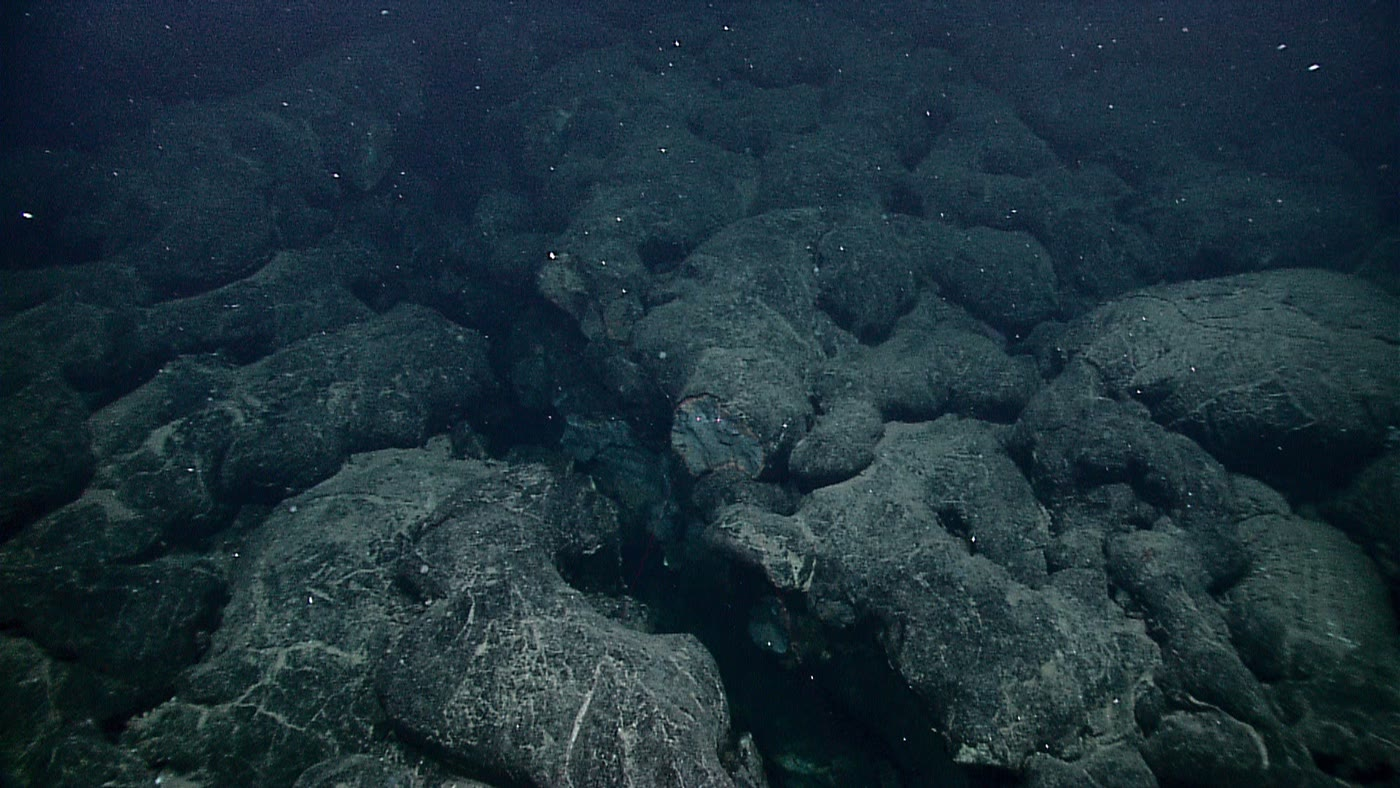
\includegraphics[width=0.6\linewidth]{images/book3/b1-pillow-lava.jpg}

\par\smallskip{\small गालापागोस दरार पर \omterm{def:b1:rifts-ridges-margins:oceanic-crust}{तकिया-लावा}, एक दरार से कटा जो उनके जमने के बाद खुला: \omterm{def:b1:rifts-ridges-margins:oceanic-crust}{महासागरीय भूपर्पटी} की परत~2 का शीर्ष जैसे-जैसे वह बनती है। हर तकिया लावा की एक जीभ है जो बाहर से समुद्र के पानी से जम गई। फ़ोटो: NOAA Okeanos Explorer Program, Galápagos Rift Expedition 2011, CC~BY~2.0 (Wikimedia Commons)।}
\label{fig:b1:rifts-ridges-margins:pillows}
\end{omfigure}
% ledger: commons:pillow-expl6453

\begin{proposition}[हर डाइक पिछले को विभाजित करता है]\label{prop:b1:rifts-ridges-margins:dykes}
मान लीजिए कि \omterm{def:b1:rifts-ridges-margins:oceanic-crust}{चादरी डाइक-संकुल} का हर डाइक प्रसार के अक्ष पर अंतर्विष्ट हुआ, जहाँ \omterm{def:b1:layered-earth:layers}{भूपर्पटी} सबसे गरम और दुर्बल है, और \omterm{def:b1:layered-earth:layers}{भूपर्पटी} अक्ष से सममित रूप से दूर खिसकती है। तब अधिकांश डाइक दो में विभाजित मिलते हैं, हर आधा अपने पुराने पड़ोसी के विरुद्ध ही ठंडे किनारे के साथ।
\end{proposition}

\begin{proof}
एक डाइक दोनों ओर की ठंडी चट्टान के विरुद्ध ठंडा होता है: बनते समय उसके दो ठंडे किनारे होते हैं। अगला डाइक वहाँ उठता है जहाँ \omterm{def:b1:layered-earth:layers}{भूपर्पटी} सबसे दुर्बल है, अक्ष के साथ, अर्थात् पिछले डाइक के बीच से, जो अब भी सबसे गरम चट्टान है। वह उसे दो हिस्सों में बाँट देता है, जिन्हें प्रसार दोनों ओर ले जाता है; हर आधे की बाहरी ओर ठंडा किनारा बना रहता है और भीतरी ओर नए डाइक के साथ बिना ठंडे हुए \omterm{def:b1:geological-maps:geological-map}{संपर्क} होता है। अंतिम को छोड़कर हर डाइक इसी तरह विभाजित होता है।
\end{proof}

एक ओर ही ठंडे किनारे वाले डाइक चादरी डाइक-संकुलों में सचमुच नियम हैं: प्रसार द्वारा बनी, डाइक-दर-डाइक बनी, एक \omterm{def:b1:layered-earth:layers}{भूपर्पटी} की पहचान।


\section{गहराई–आयु नियम}\label{sec:b1:rifts-ridges-margins:depth-age}

महासागर-तल कटक पर उथला और उससे दूर गहरा है। चूँकि तल कटक पर बनता है और दूर ले जाया जाता है, कटक से दूरी आयु है, और तल की गहराई उसकी आयु पर निर्भर करती है। प्लेट बूढ़ी होते हुए ऊपर से ठंडी होती है (\cref{ch:b1:heat-budget}); ठंडी चट्टान सघनतर होती है, और एक सघनतर स्तंभ नीचे तैरता है।

\begin{lemma}[त्रुटि-फलन का एक समाकल]\label{lem:b1:rifts-ridges-margins:erfc}
$\operatorname{erfc} u = 1 - \operatorname{erf} u =
\frac{2}{\sqrt\pi}\int_u^\infty e^{-s^2}\,\mathrm ds$ के साथ,
\[
  \int_0^\infty \operatorname{erfc} u \,\mathrm du = \frac{1}{\sqrt\pi}.
\]
\end{lemma}

\begin{proof}
$\operatorname{erfc}$ का अवकलज $-\frac{2}{\sqrt\pi}e^{-u^2}$ है। $[0, X]$ पर खंडशः समाकलन करने पर,
\[
  \int_0^X \operatorname{erfc} u\,\mathrm du
  = \bigl[u \operatorname{erfc} u\bigr]_0^X + \frac{2}{\sqrt\pi}\int_0^X u\,e^{-u^2}\,\mathrm du
  = X\operatorname{erfc} X + \frac{1}{\sqrt\pi}\bigl(1 - e^{-X^2}\bigr).
\]
$X > 0$ और $s \ge X$ के लिए, $e^{-s^2} \le (s/X)e^{-s^2}$, अतः
$X\operatorname{erfc} X \le \frac{2}{\sqrt\pi}\int_X^\infty s\,e^{-s^2}\,\mathrm ds
= e^{-X^2}/\sqrt\pi$, जो 0 की ओर जाता है। $X \to \infty$ देने पर परिणाम मिलता है।
\end{proof}

\begin{theorem}[गहराई–आयु नियम]\label{thm:b1:rifts-ridges-margins:depth-age}
मान लीजिए कि
\begin{enumerate}
  \item \omterm{def:b1:layered-earth:layers}{प्रावार} एकसमान तापमान $T_m$ पर कटक छोड़ता है, और आयु $t$ की महासागरीय प्लेट एक अर्ध-अंतरिक्ष है जो तब से अपनी सतह से ठंडा हुआ है, जो $T_0$ पर रखी है, ऊष्मीय विसरणशीलता $\kappa$ के साथ;
  \item ठंडी चट्टान का घनत्व $\rho_m\bigl(1 + \alpha(T_m -
        T)\bigr)$ है, जहाँ $\rho_m$, $T_m$ पर \omterm{def:b1:layered-earth:layers}{प्रावार} का घनत्व है और $\alpha$ उसका ऊष्मीय प्रसार-गुणांक;
  \item हर स्तंभ एक \omterm{def:b1:isostasy-gravity:isostasy}{प्रतिपूर्ति गहराई} के ऊपर समस्थैतिक साम्य में है जो ठंडी परत के नीचे है, और समुद्री पानी का घनत्व $\rho_w$ है।
\end{enumerate}
तब आयु $t$ के समुद्र-तल की गहराई है
\[
  d(t) = d_r + C\sqrt t, \qquad
  C = \frac{2}{\sqrt\pi}\,\frac{\rho_m\,\alpha\,(T_m - T_0)\sqrt\kappa}{\rho_m - \rho_w},
\]
जहाँ $d_r$ कटक-अक्ष की गहराई है। यह महासागर-तल का \emph{गहराई–आयु नियम}\index{गहराई–आयु नियम} है।
\end{theorem}

\begin{proof}
ठंडे अर्ध-अंतरिक्ष में तापमान है
\[
  T(z, t) = T_0 + (T_m - T_0)\operatorname{erf}\frac{z}{2\sqrt{\kappa t}},
\]
जहाँ $z$ समुद्र-तल के नीचे गहराई है; ऊष्मा-समीकरण का यह हल, जैसा \cref{ch:b1:heat-budget} में, यहाँ स्वीकृत है, और पुस्तक 5 में व्युत्पन्न होता है। कटक पर का स्तंभ तुलना कीजिए, जो $d_r$ तक पानी और नीचे $T_m$ पर \omterm{def:b1:layered-earth:layers}{प्रावार} से बना है, आयु $t$ के स्तंभ से, जो $d$ तक पानी और नीचे ठंडी प्लेट से बना है, दोनों \omterm{def:b1:isostasy-gravity:isostasy}{प्रतिपूर्ति गहराई} $D$ तक। उनके प्रति एकाई क्षेत्रफल द्रव्यमान बराबर हैं:
\[
  \rho_w d_r + \rho_m (D - d_r) = \rho_w d + \int_0^{D-d}\rho_m\bigl(1 + \alpha(T_m - T)\bigr)\mathrm dz
  = \rho_w d + \rho_m (D - d) + \rho_m\alpha\int_0^{D-d}(T_m - T)\,\mathrm dz.
\]
अतः
\[
  (\rho_m - \rho_w)(d - d_r) = \rho_m\alpha\int_0^{D-d}(T_m - T)\,\mathrm dz.
\]
चूँकि $T_m - T = (T_m - T_0)\operatorname{erfc}\bigl(z/2\sqrt{\kappa t}\bigr)$ ठंडी परत के नीचे नगण्य है, समाकल को अनंत तक लिया जा सकता है; $u = z/2\sqrt{\kappa t}$ और \cref{lem:b1:rifts-ridges-margins:erfc} के साथ,
\[
  \int_0^\infty (T_m - T)\,\mathrm dz = (T_m - T_0)\,2\sqrt{\kappa t}\int_0^\infty\operatorname{erfc}u\,\mathrm du
  = \frac{2}{\sqrt\pi}(T_m - T_0)\sqrt{\kappa t}.
\]
$\rho_m - \rho_w$ से भाग देने पर $d - d_r = C\sqrt t$ मिलता है।
\end{proof}

पानी मायने रखता है: जैसे-जैसे प्लेट धँसती है, पानी उसके ऊपर का स्थान भरता है, और उसका भार उसे और नीचे दबाता है। प्रभावी प्रसार-गुणांक $\alpha\rho_m/(\rho_m - \rho_w)$ है, जो $\alpha$ से गुणनखंड $3300/2300 \approx 1.43$ द्वारा बड़ा है।

$\alpha = \qty{3.2e-5}{K^{-1}}$, $T_m - T_0 = \qty{1350}{K}$,
$\kappa = \qty{e-6}{m^2.s^{-1}}$, $\rho_m = \qty{3300}{kg.m^{-3}}$ और
$\rho_w = \qty{1000}{kg.m^{-3}}$ के साथ, और समय दस लाख वर्षों में गिनते हुए ($\sqrt{\kappa\times\qty{1}{Myr}} = \qty{5618}{m}$), प्रमेय $C = \qty{393}{m.Myr^{-1/2}}$ देता है। पार्सन्स और स्क्लेटर ने उत्तरी प्रशांत और उत्तरी अटलांटिक की गहराइयों से, तलछट हटाने के बाद, जो स्थिरांक निकाले, वे निकट हैं: $d_r \approx \qty{2500}{m}$ और $C \approx \qty{350}{m.Myr^{-1/2}}$, 0 से \qty{70}{Myr} तक। ऊपर प्रयुक्त $\alpha$ और $T_m$ के मान उनके पुराने तल के प्लेट-प्रतिरूप के हैं, \qty{1350}{\degreeCelsius} पर \omterm{def:b1:layered-earth:layers}{प्रावार} और $\alpha = \qty{3.2e-5}{\per\degreeCelsius}$, जो क्रमशः एक-पाँचवें और एक-तिहाई तक अनिश्चित हैं, अतः 393 और 350 का मेल जितना हो सकता था उतना अच्छा है।
% ledger: parsons:plate-model, ps77:depth-age

\begin{example}[महासागर-तल 25 और 100 मिलियन वर्ष पुराना]\label{ex:b1:rifts-ridges-margins:depths}
$d = 2500 + 350\sqrt t$ के साथ (मीटर में, $t$ मिलियन वर्षों में), \qty{25}{Myr} पुराना तल $2500 + 350\times5 = \qty{4250}{m}$ पर और \qty{100}{Myr} पुराना तल $2500 + 350\times10 = \qty{6000}{m}$ पर है। तल अपने पहले 25 मिलियन वर्षों में \qty{1750}{m} धँसता है, और अगले 75 में बस \qty{1750}{m} और।
\end{example}
% ledger: parsons:plate-model

\begin{omfigure}
\begin{tikzpicture}
\begin{axis}[omrecord, omdepth, width=0.84\linewidth, height=6.6cm,
  xmin=0, xmax=13.6, ymin=2000, ymax=6800,
  xlabel={तल की आयु का वर्गमूल, $\sqrt t$ (\unit{Myr^{1/2}})},
  ylabel={गहराई (\unit{m})},
  yticklabel style={/pgf/number format/set thousands separator={}},
  legend style={font=\scriptsize, at={(0.02,0.03)}, anchor=south west, draw=none, fill=white, fill opacity=0.85, text opacity=1},
  legend cell align=left]
% computed in figdata/bachelor-1/depth_age.py; ledger: data:etopo1, data:b2-seafloor-age, parsons:plate-model
\addplot[name path=lo, draw=none, forget plot] table[x expr=sqrt(\thisrow{t}), y=q1] {figdata/out/bachelor-1-depth_age-bins.dat};
\addplot[name path=hi, draw=none, forget plot] table[x expr=sqrt(\thisrow{t}), y=q3] {figdata/out/bachelor-1-depth_age-bins.dat};
\addplot[black!12] fill between[of=lo and hi];
\addlegendentry{कोषों का बीच का आधा}
\addplot[only marks, mark=*, mark size=1.1pt, black!70] table[x expr=sqrt(\thisrow{t}), y=median] {figdata/out/bachelor-1-depth_age-bins.dat};
\addlegendentry{माध्यिका गहराई, 2-\unit{Myr} आयु-वर्ग}
\addplot[very thick, omProp] table[x expr=sqrt(\thisrow{t}), y=halfspace] {figdata/out/bachelor-1-depth_age-models.dat};
\addlegendentry{अर्ध-अंतरिक्ष, $2500 + 350\sqrt t$}
\addplot[thick, omDef, densely dashed] table[x expr=sqrt(\thisrow{t}), y=plate] {figdata/out/bachelor-1-depth_age-models.dat};
\addlegendentry{प्लेट प्रतिरूप, $6400 - 3200\,e^{-t/62.8}$}
\draw[black!50, densely dotted] (axis cs:8.944,2000) -- (axis cs:8.944,6800);
\node[font=\scriptsize, anchor=north west, black!70] at (axis cs:8.944,2060) {\qty{80}{Myr}};
\node[font=\scriptsize, anchor=north west, black!70] at (axis cs:4.472,2060) {\qty{20}{Myr}};
\draw[black!50, densely dotted] (axis cs:4.472,2000) -- (axis cs:4.472,6800);
\end{axis}
\end{tikzpicture}

\par\smallskip{\small समुद्र-तल की गहराई उसकी आयु के वर्गमूल के विरुद्ध। हर बिंदु एक-डिग्री कोषों की माध्यिका गहराई है जिनका तल दो-मिलियन-वर्ष आयु-वर्ग में आता है (31\,538 कोष, \qty{1000}{m} से गहरे); धूसर पट्टी उनमें बीच का आधा रखती है। अर्ध-अंतरिक्ष नियम इस आलेख में एक सीधी रेखा है। युवा तल उसका निकटता से अनुसरण करता है; पुराना तल उसके ऊपर है, क्योंकि कोष अपने अवसाद साथ रखते हैं और समुद्री पर्वत तथा ज्वालामुखी पठार शामिल हैं, और क्योंकि पुराना तल धँसना बंद कर देता है (बिंदुकित रेखा: प्लेट प्रतिरूप)। डेटा: ETOPO1 (NOAA) और Seton और अन्य (2020) की समुद्र-तल आयु।}
\label{fig:b1:rifts-ridges-margins:depth-age}
\end{omfigure}

यह आलेख पूरे महासागर पर प्रमेय की परख करता है। लगभग \qty{20}{Myr} ($\sqrt t \approx 4.5$) तक माध्यिकाएँ नियम से लगभग सौ मीटर के भीतर पड़ती हैं। \qty{70}{Myr} से युवा माध्यिकाओं पर फ़िट सीधी रेखा की ढलान केवल \qty{250}{m.Myr^{-1/2}} है: मापी गई गहराइयाँ अवसाद की सतह की हैं, जबकि नियम \omterm{def:b1:layered-earth:layers}{भूपर्पटी} के शीर्ष की गहराई देता है, और अवसाद का आवरण आयु के साथ मोटा होता है। 60 और \qty{80}{Myr} के बीच, अवसाद हटाने के बाद भी तल वर्गमूल-नियम से विचलित होता है: वह नियम से उथला हो जाता है, और धँसना बंद कर देता है।
प्लेट प्रतिरूप, \qty{125}{km} मोटी एक प्लेट जिसका आधार \omterm{def:b1:layered-earth:layers}{प्रावार} के तापमान पर रखा गया है, इस चपटेपन का वर्णन करता है: उसकी गहराई लगभग \qty{6400}{m} की ओर जाती है, और उसका \omterm{def:b1:heat-budget:heat-flow}{ऊष्मा-प्रवाह} एक स्थिरांक की ओर, मानो संवहन करते \omterm{def:b1:layered-earth:layers}{प्रावार} ने पुरानी प्लेटों के आधार पर ऊष्मा पहुँचाई हो। वह प्रतिरूप पुस्तक 5 में पढ़ा जाता है; इस पुस्तक में वर्गमूल नियम \qty{80}{Myr} तक प्रयुक्त होता है।
% ledger: parsons:plate-model; fit and cell count from depth_age.py (values part)

\begin{method}[तल की गहराई से उसकी आयु निर्धारण]\label{met:b1:rifts-ridges-margins:age-from-depth}
समुद्र-तल की आयु का अनुमान लगाने के लिए, जहाँ उसकी चुंबकीय विसंगतियाँ अनुपस्थित हैं या मानचित्रित नहीं हैं:
\begin{enumerate}
  \item तल की गहराई मापिए और भूकंपीय परिच्छेदों से उसके अवसादों की मोटाई; \omterm{def:b1:layered-earth:layers}{भूपर्पटी} के शीर्ष की गहराई $d$ लीजिए, अवसादों के भार के लिए सुधारी हुई;
  \item नियम को उलटिए: $t = \bigl((d - d_r)/C\bigr)^2$, संबंधित महासागर के लिए $d_r$ और $C$ के साथ;
  \item जाँचिए कि तल \qty{80}{Myr} से युवा है, और अनिश्चितता का अनुमान लगाइए: गहराई पर त्रुटि $\delta d$ देती है $\delta t = 2t\,\delta d/(d - d_r)$।
\end{enumerate}
\end{method}

\qty{4600}{m} पर तल के लिए, $t = (2100/350)^2 = \qty{36}{Myr}$, और गहराई पर \qty{100}{m} की अनिश्चितता आयु पर $2\times36\times100/2100 \approx
\qty{3.4}{Myr}$ देती है। जहाँ तल एक व्यापक क्षेत्र पर नियम की भविष्यवाणी से उथला है, एक उभार, तो कारण आयु नहीं बल्कि नीचे से ऊष्मा है (\cref{ch:b1:hotspots})।

नियम महासागर को समुद्र-तल से भी जोड़ता है। एक कटक जो तेज़ फैलता है, युवा, उथला तल अपने अक्ष से दूर ले जाता है; महासागर द्रोणियों में कम पानी रखते हैं, और समुद्र महाद्वीपों पर चढ़ता है। दसियों मिलियन वर्षों में, प्रसार-दर में परिवर्तन विश्वव्यापी समुद्र-स्तर परिवर्तनों के दो मुख्य कारणों में से एक है, जिसके साथ भूमि पर बर्फ़ की मात्रा है।

\section{रूपांतर भ्रंश और भंग-क्षेत्र}

कटक निरंतर रेखाएँ नहीं हैं: वे खंडों में कटे हैं जो उनके समकोण पर चलने वाले भ्रंशों से विस्थापित हैं, प्रसार की दिशा के अनुदिश। विस्थापनों से आगे, भ्रंश महासागर-तल पर लंबे निशानों के रूप में जारी रहते हैं।

\begin{definition}[रूपांतर भ्रंश, भंग-क्षेत्र]\label{def:b1:rifts-ridges-margins:transform}
एक \emph{रूपांतर भ्रंश}\index{रूपांतर भ्रंश} एक क्षैतिज-सरकने वाला भ्रंश है जो एक प्लेट-सीमा है और अन्य प्लेट-सीमाओं पर समाप्त होता है; एक कटक–कटक रूपांतर दो विस्थापित कटक-खंडों के सिरों को जोड़ता है। एक \emph{भंग-क्षेत्र}\index{भंग-क्षेत्र} कटक-खंडों के सिरों से परे रूपांतर भ्रंश की निरंतरता है: महासागर-तल के पार एक रैखिक घाटी या सीढ़ी, जो एक ही प्लेट से संबंधित भिन्न आयु के तल को अलग करती है।
\end{definition}

\begin{proposition}[कटक–कटक रूपांतर पर विस्थापन]\label{prop:b1:rifts-ridges-margins:transform}
दो कटक-खंड, जो अपने-अपने लंबवत, अर्ध दर $u$ पर सममित रूप से फैलते हैं, लंबाई $a$ के एक \omterm{def:b1:rifts-ridges-margins:transform}{रूपांतर भ्रंश} द्वारा विस्थापित हैं। तब:
\begin{enumerate}
  \item रूपांतर के दोनों पक्ष एक-दूसरे के पार पूर्ण दर $2u$ पर सरकते हैं, उस दिशा के उल्टे में जो \omterm{def:b1:cross-sections:throw}{विस्थापन} सुझाता यदि एक सीधा कटक काटा गया होता और भ्रंश द्वारा हटाया गया होता;
  \item भंग-क्षेत्रों के अनुदिश दोनों पक्ष एक-दूसरे के सापेक्ष नहीं चलते, और दोनों ओर का तल आयु में $a/u$ से भिन्न है;
  \item रूपांतर की लंबाई समय के साथ नहीं बदलती।
\end{enumerate}
\end{proposition}

\begin{proof}
फ़्रेम में कटक के संदर्भ में, रूपांतर के अनुदिश पूर्व की ओर $x$ अक्ष, और उत्तर की ओर $y$ अक्ष लीजिए। उत्तरी खंड $x = 0$, $y > 0$ पर हो, और दक्षिणी $x = a$, $y < 0$ पर (\omterm{def:b1:cross-sections:throw}{विस्थापन} दक्षिण जाते हुए पूर्व की ओर है); रूपांतर, $0 < x < a$ का, $y = 0$ पर खंड है। पश्चिमी प्लेट $W$ दोनों खंडों के पश्चिम में है और $-u$ पर, $x$ के अनुदिश, चलती है; पूर्वी प्लेट $E$ दोनों के पूर्व में है और $+u$ पर चलती है।

(1) रूपांतर के ठीक उत्तर में, $0 < x < a$ पर, तल उत्तरी खंड के पूर्व में है: वह $E$ का है और $u$ पर पूर्व की ओर चलता है। उसके ठीक दक्षिण में, तल दक्षिणी खंड के पश्चिम में है: वह $W$ का है और $u$ पर पश्चिम की ओर चलता है। उत्तरी पक्ष दक्षिणी पक्ष के सापेक्ष $2u$ पर पूर्व की ओर चलता है: किसी भी पक्ष से देखने पर दूर का पक्ष दाहिनी ओर चलता है, और सरकाव दाहिने-पार्श्व है। भ्रंश द्वारा काटा गया एक सीधा कटक, जिसका दक्षिणी भाग अब उत्तरी भाग के पूर्व में है, इसके बजाय एक बाएँ-पार्श्व \omterm{def:b1:cross-sections:throw}{विस्थापन} दर्ज करता।

(2) $x > a$ के लिए, दोनों पक्ष अपने खंडों के पूर्व में हैं और $E$ के हैं: वे एक साथ चलते हैं। उत्तरी खंड से दूरी $x$ पर, \omterm{def:b1:rifts-ridges-margins:transform}{भंग-क्षेत्र} के उत्तर का तल आयु $x/u$ का है; उसके दक्षिण का तल दक्षिणी खंड से $x - a$ पर है और उसकी आयु $(x - a)/u$ है। अंतर $a/u$ है। वही $x < 0$ के लिए धारण करता है, जहाँ दोनों पक्ष $W$ के हैं।

(3) दोनों खंड कटक के फ़्रेम में $x = 0$ और $x = a$ पर रहते हैं, क्योंकि हर एक सममित रूप से फैलता है: रूपांतर लंबाई $a$ रखता है।
\end{proof}

जे॰\ टूज़ो विल्सन ने 1965 में देखा कि कटकों के \omterm{def:b1:cross-sections:throw}{विस्थापन} एक पुराने, सीधे कटक के \omterm{def:b1:cross-sections:throw}{विस्थापन} के रूप में नहीं पढ़े जा सकते, और उन्होंने प्रमेय की विस्थापन-दिशा की भविष्यवाणी की; रूपांतरों पर भूकंपों के फ़ोकल मैकेनिज़्म ने इसकी पुष्टि की। भूकंप सक्रिय रूपांतर के साथ होते हैं, कटक के सिरों के बीच; \omterm{def:b1:rifts-ridges-margins:transform}{भंग-क्षेत्र} आम तौर पर शांत होते हैं। \omterm{def:b1:rifts-ridges-margins:transform}{भंग-क्षेत्र} के आर-पार दोनों पक्षों के तल की आयु भिन्न है, अतः \omterm{thm:b1:rifts-ridges-margins:depth-age}{गहराई–आयु नियम} के अनुसार भिन्न गहराई: एक ऐसी सीढ़ी जो कटक से दूरी के साथ धीरे-धीरे लुप्त होती है। उत्तरी अटलांटिक में, लगभग \ang{52}\,N पर, दो चार्ली–गिब्स रूपांतर मध्य-अटलांटिक कटक को कुल मिलाकर लगभग \qty{350}{km} विस्थापित करते हैं।
% ledger: wilson:transform, data:pb2002 (offset summed over the transform steps in figdata/bachelor-1/ridge_budget.py)

\begin{omfigure}
\begin{tikzpicture}[x=0.95cm, y=0.95cm, font=\scriptsize]
\fill[omSea!10] (-5,-2.6) rectangle (8,2.6);
% isochrons (10 and 20 Myr), offset across the fracture zones
\foreach \x in {-4,-2,2,4} \draw[black!40] (\x,0) -- (\x,2.5);
\foreach \x in {-1,1,5,7} \draw[black!40] (\x,0) -- (\x,-2.5);
\node[black!55, anchor=south, fill=omSea!10, inner sep=1pt] at (2,2.0) {10};
\node[black!55, anchor=south, fill=omSea!10, inner sep=1pt] at (4,2.0) {20};
\node[black!55, anchor=south, fill=omSea!10, inner sep=1pt] at (-2,2.0) {10};
\node[black!55, anchor=south, fill=omSea!10, inner sep=1pt] at (-4,2.0) {20};
\node[black!55, anchor=north, fill=omSea!10, inner sep=1pt] at (5,-2.0) {10};
\node[black!55, anchor=north, fill=omSea!10, inner sep=1pt] at (7,-2.0) {20};
\node[black!55, anchor=north, fill=omSea!10, inner sep=1pt] at (1,-2.0) {10};
\node[black!55, anchor=north, fill=omSea!10, inner sep=1pt] at (-1,-2.0) {20};
% fracture zones and transform
\draw[black!60, thick, densely dashed] (-5,0) -- (0,0);
\draw[black!60, thick, densely dashed] (3,0) -- (8,0);
\draw[transform, line width=1.4pt] (0,0) -- (3,0);
% ridge segments
\draw[ridge, line width=1.1pt] (0,0) -- (0,2.6);
\draw[ridge, line width=1.1pt] (3,0) -- (3,-2.6);
\pic at (1.5,0) {dextral={90}};
\foreach \x in {0.4,0.75,2.25,2.6} \node[star, star points=5, star point ratio=2.2, fill=orange!90!black, draw=black, line width=0.2pt, inner sep=1.5pt] at (\x,0.0) {};
% plate motions
\draw[-{Stealth[length=4pt]}, very thick, black!70] (-2.8,1.1) -- (-3.9,1.1);
\draw[-{Stealth[length=4pt]}, very thick, black!70] (-0.2,-1.1) -- (-1.3,-1.1);
\draw[-{Stealth[length=4pt]}, very thick, black!70] (5.5,1.1) -- (6.6,1.1);
\draw[-{Stealth[length=4pt]}, very thick, black!70] (5.3,-1.1) -- (6.4,-1.1);
\node[font=\small] at (-3.3,1.55) {प्लेट $W$};
\node[font=\small] at (6.1,1.55) {प्लेट $E$};
\node[anchor=west, omRidge] at (0.1,2.25) {कटक};
\node[anchor=east, omRidge] at (2.9,-2.25) {कटक};
\node[anchor=north, align=center, fill=white, fill opacity=0.8, text opacity=1, inner sep=1pt] at (1.5,-0.35) {रूपांतर भ्रंश\\(सक्रिय, भूकंप)};
\node[anchor=south, fill=white, fill opacity=0.8, text opacity=1, inner sep=1pt] at (5.5,0.12) {भंग-क्षेत्र (निष्क्रिय)};
\node[anchor=north, fill=white, fill opacity=0.8, text opacity=1, inner sep=1pt] at (-2.5,-0.12) {भंग-क्षेत्र (निष्क्रिय)};
\node[anchor=south, black!70, fill=omSea!10, inner sep=1pt] at (6.2,0.55) {पुराना, गहरा};
\node[anchor=north, black!70, fill=omSea!10, inner sep=1pt] at (6.0,-0.45) {युवा, उथला};
\end{tikzpicture}

\par\smallskip{\small एक कटक, जो एक \omterm{def:b1:rifts-ridges-margins:transform}{रूपांतर भ्रंश} से विस्थापित है, मानचित्र दृश्य में, उत्तर ऊपर। दोनों प्लेटें हर खंड से दूर चलती हैं (काले तीर); रूपांतर (लाल) के साथ वे दाहिने-पार्श्व एक-दूसरे को सरकाती हैं (अर्ध-तीर), यद्यपि कटक का \omterm{def:b1:cross-sections:throw}{विस्थापन} बाएँ-पार्श्व दिखता है। धूसर रेखाएँ समसमयिक रेखाएँ हैं, लाखों वर्षों में नामांकित: हर \omterm{def:b1:rifts-ridges-margins:transform}{भंग-क्षेत्र} (बिंदुकित) के आर-पार भिन्न आयु का तल, अतः भिन्न गहराई, साथ-साथ पड़ता है, पर दोनों पक्ष एक साथ चलते हैं। तारे: भूकंप, केवल रूपांतर तक सीमित।}
\label{fig:b1:rifts-ridges-margins:transform}
\end{omfigure}

रूपांतर \cref{ch:b1:plate-kinematics} की प्लेट गतियों के लिए साक्ष्य का तीसरा प्रकार हैं: एक रूपांतर दोनों प्लेटों के सापेक्ष वेग के अनुदिश चलता है, इसलिए वह उनके \omterm{def:b1:plate-kinematics:euler-pole}{यूलर ध्रुव} के परितः एक लघुवृत्त पर स्थित है, और कई रूपांतरों के लंबवत खींचे गए \omterm{def:b1:spherical-astronomy:spherical-triangle}{महावृत्त} ध्रुव पर मिलते हैं। \omterm{def:b1:rifts-ridges-margins:transform}{भंग-क्षेत्र}, महासागर-तल के पार खींचे गए, अतीत में गति की दिशा दर्ज करते हैं, जैसे चुंबकीय विसंगतियाँ उसकी दर दर्ज करती हैं।

\section{अभ्यास}

\begin{exercise}[$\star$]\label{exo:b1:rifts-ridges-margins:1}
2005 में अफ़ार दरार का एक \qty{60}{km} लंबा खंड \qty{8}{m} तक खुला, और \qty{2.5}{km^3} मैग्मा अंतर्विष्ट हुआ। (क) यदि डाइक पूरे खंड में \qty{8}{m} मोटा होता, तो उसकी औसत ऊँचाई क्या होती? (ख) \qty{18}{mm.yr^{-1}} की प्लेट दर पर, \qty{8}{m} का खुलाव कितने वर्षों की गति दर्शाता है?
% ledger: wright:afar, morvel:ar-nb
\end{exercise}

\begin{exercise}[$\star$]\label{exo:b1:rifts-ridges-margins:2}
एक \omterm{def:b1:rifts-ridges-margins:rift}{अर्ध-ग्राबेन} की सीमा एक \ang{60} \omterm{def:b1:geological-maps:attitude}{नति} वाले, \qty{3.0}{km} \omterm{def:b1:cross-sections:throw}{विस्थापन} के सीमा-भ्रंश से बंधी है, और उसे \ang{70} \omterm{def:b1:geological-maps:attitude}{नति} वाले, \qty{0.8}{km} \omterm{def:b1:cross-sections:throw}{विस्थापन} के एक छोटे प्रतिविलोम भ्रंश ने काटा है। (क) हर भ्रंश का \omterm{def:b1:cross-sections:throw}{क्षैतिज विस्थापन} और खंड का विस्तार परिकलित कीजिए। (ख) खंड अब \qty{25}{km} चौड़ा है: भ्रंशन से पहले वह कितना चौड़ा था?
\end{exercise}

\begin{exercise}[$\star$]\label{exo:b1:rifts-ridges-margins:3}
परिभाषा की सीमाओं से, प्लेट सदिशों से परिकलित उनकी पूर्ण प्रसार-दरों के आधार पर इन कटकों का वर्गीकरण कीजिए: गाक्कल कटक \qty{12}{mm.yr^{-1}}; मध्य लाल सागर \qty{15}{mm.yr^{-1}}; रेक्यनीस कटक \qty{19}{mm.yr^{-1}}; पश्चिमी कार्ल्सबर्ग कटक \qty{23}{mm.yr^{-1}}; दक्षिण अटलांटिक पर \ang{20}\,S \qty{33}{mm.yr^{-1}}; पूर्वी प्रशांत उभार पर \ang{20}\,S \qty{143}{mm.yr^{-1}}। उनमें से किसमें अक्षीय घाटी की आप अपेक्षा करेंगे, और किसमें अक्षीय उभार?
% ledger: morvel:eu-na, morvel:redsea, morvel:in-sm, morvel:nb-sa, morvel:nz-pa (rates computed with euler_velocities.py)
\end{exercise}

\begin{exercise}[$\star$]\label{exo:b1:rifts-ridges-margins:4}
हर वर्ष लगभग \qty{3.0}{km^2} नया महासागर-तल बनता है, \qty{7.1}{km} मोटी \omterm{def:b1:layered-earth:layers}{भूपर्पटी} के साथ। (क) हर वर्ष कितनी \omterm{def:b1:layered-earth:layers}{भूपर्पटी} का आयतन बनता है? (ख) इस दर पर, \qty{3.028e8}{km^2} महासागर-तल बनाने में कितना समय लगेगा? उसकी तुलना सबसे पुराने महासागर-तल की आयु, लगभग \qty{190}{Myr}, से कीजिए, और समझाइए कि दोनों सहमत क्यों होने ज़रूरी नहीं।
% ledger: data:pb2002 (ridge_budget.py), white:crust, dd10:split, data:b2-seafloor-age
\end{exercise}

\begin{exercise}[$\star\star$]\label{exo:b1:rifts-ridges-margins:5}
$d = 2500 + 350\sqrt t$ के साथ (मीटर में, $t$ मिलियन वर्षों में): (क) 4, 36 और 64 मिलियन वर्ष पुराने तल की गहराई परिकलित कीजिए; (ख) \qty{4600}{m} और \qty{5300}{m} पर स्थित तल की आयु ज्ञात कीजिए; (ग) 4 और \qty{36}{Myr} के बीच, और 36 और \qty{64}{Myr} के बीच, तल कितना धँसता है?
\end{exercise}

\begin{exercise}[$\star\star$]\label{exo:b1:rifts-ridges-margins:6}
\omterm{thm:b1:rifts-ridges-margins:depth-age}{गहराई–आयु नियम} (\cref{thm:b1:rifts-ridges-margins:depth-age}) का स्थिरांक $C$ परिकलित कीजिए, $\alpha =
\qty{3.2e-5}{K^{-1}}$, $\rho_m = \qty{3300}{kg.m^{-3}}$, $\rho_w =
\qty{1000}{kg.m^{-3}}$, $T_m - T_0 = \qty{1350}{K}$ और $\kappa =
\qty{e-6}{m^2.s^{-1}}$ के साथ, \unit{m.Myr^{-1/2}} में। उसे \qty{250}{K} ठंडे \omterm{def:b1:layered-earth:layers}{प्रावार} के लिए फिर से परिकलित कीजिए। एक ठंडे महासागर का तल किस स्थिरांक का अनुसरण करेगा?
% ledger: parsons:plate-model
\end{exercise}

\begin{exercise}[$\star\star$]\label{exo:b1:rifts-ridges-margins:7}
प्लेट प्रतिरूप महासागर-तल की \omterm{def:b1:heat-budget:heat-flow}{ऊष्मा-प्रवाह} को $q = 11.3/\sqrt t$ देता है, \qty{e-6}{cal.cm^{-2}.s^{-1}} की इकाइयों में, $t$ मिलियन वर्षों में। (क) स्थिरांक को \unit{mW.m^{-2}.Myr^{1/2}} में बदलिए ($\qty{1}{cal} =
\qty{4.184}{J}$) और उसकी तुलना \cref{ch:b1:heat-budget} के \qty{490}{mW.m^{-2}.Myr^{1/2}} से कीजिए। (ख) \qty{1}, \qty{10} और \qty{150}{Myr} पर $q$ परिकलित कीजिए। नियम \qty{120}{Myr} तक पुराने तल पर फ़िट किया गया था, और प्लेट प्रतिरूप पुराने तल के \omterm{def:b1:heat-budget:heat-flow}{ऊष्मा-प्रवाह} को एक स्थिरांक पर समतल करता है: \qty{150}{Myr} पर उसका मान तब बहुत ऊँचा है या बहुत नीचा?
% ledger: parsons:plate-model, dd10:young-ocean
\end{exercise}

\begin{exercise}[$\star\star$]\label{exo:b1:rifts-ridges-margins:8}
एक उत्तर–दक्षिण प्रवृत्ति वाला कटक दो खंडों में कटा है; कटक के साथ दक्षिण जाते हुए, एक \omterm{def:b1:rifts-ridges-margins:transform}{रूपांतर भ्रंश} पर अक्ष \qty{40}{km} \emph{पश्चिम} की ओर कूदता है। (क) रूपांतर पर सरकाव की दिशा क्या है? (ख) कटक का \omterm{def:b1:cross-sections:throw}{विस्थापन} क्या दिखाता प्रतीत होता है? (ग) रूपांतर की रेखा के किस भाग के अनुदिश भूकंप होते हैं, और आगे क्यों नहीं?
\end{exercise}

\begin{exercise}[$\star\star$]\label{exo:b1:rifts-ridges-margins:9}
चार्ली–गिब्स \omterm{def:b1:rifts-ridges-margins:transform}{भंग-क्षेत्र} मध्य-अटलांटिक कटक को कुल मिलाकर \qty{350}{km} विस्थापित करते हैं; वहाँ \omterm{def:b1:plate-kinematics:spreading-rate}{पूर्ण प्रसार-दर} \qty{21.2}{mm.yr^{-1}} है। \omterm{def:b1:cross-sections:throw}{विस्थापन} को एक एकल रूपांतर मानिए। (क) \omterm{def:b1:rifts-ridges-margins:transform}{भंग-क्षेत्र} के आर-पार आयु में अंतर क्या है? (ख) $d = 2500 + 350\sqrt t$ के प्रयोग से, रूपांतर के अंत पर, फिर उससे आगे \qty{100}{km} और \qty{1000}{km} पर \omterm{def:b1:rifts-ridges-margins:transform}{भंग-क्षेत्र} के आर-पार गहराई का चरण परिकलित कीजिए।
% ledger: data:pb2002 (ridge_budget.py), morvel:eu-na (rate at 52.5 N 31.5 W from euler_velocities.py)
\end{exercise}

\begin{exercise}[$\star\star\star$]\label{exo:b1:rifts-ridges-margins:10}
एक महासागर द्रोणी एक स्थिर दर पर बनती है और हर आयु का तल समान क्षेत्रफलों में रखती है, 0 से $A$ तक। (क) दिखाइए कि उसकी माध्य गहराई $d_r +
\frac23C\sqrt A$ है। (ख) $d_r = \qty{2500}{m}$ और $C = \qty{350}{m.Myr^{-1/2}}$ के साथ, $A = \qty{180}{Myr}$ और
$A = \qty{120}{Myr}$ की तुलना कीजिए। (ग) यदि द्रोणी का प्रसार तेज़ हो जाए ताकि उसका सबसे पुराना तल \qty{180}{Myr} के बजाय \qty{120}{Myr} हो, तो समुद्र-स्तर कितना बढ़ता है, महाद्वीपों की बाढ़ नगण्य मानते हुए, पर तल पर अतिरिक्त पानी के भार को ध्यान में रखते हुए, जो उन्नयन का $\rho_w/(\rho_m - \rho_w)$ गुना धँसता है ($\rho_m = 3300$, $\rho_w = \qty{1000}{kg.m^{-3}}$)?
\end{exercise}

\begin{exercise}[$\star\star\star$]\label{exo:b1:rifts-ridges-margins:11}
\cref{prop:b1:rifts-ridges-margins:transform} के संदर्भ में, दूर वाले कटक खंड से दूरी $x > a$ पर \omterm{def:b1:rifts-ridges-margins:transform}{भंग-क्षेत्र} के आर-पार गहराई का चरण $\Delta d = C\bigl(\sqrt{x/u} - \sqrt{(x - a)/u}\bigr)$ है। (क) दिखाइए कि $x \gg a$ के लिए, $\Delta d \approx Ca/(2\sqrt{ux})$। (ख) $C = \qty{350}{m.Myr^{-1/2}}$, $a = \qty{350}{km}$ और $u = \qty{10.6}{km.Myr^{-1}}$ के साथ, $x = 450$, 1350 और \qty{3350}{km} पर सटीक और सन्निकट चरणों की तुलना कीजिए। सन्निकटन कब \qty{10}{\percent} तक अच्छा है?
\end{exercise}

\begin{exercise}[$\star\star\star$]\label{exo:b1:rifts-ridges-margins:12}
अर्ध-अंतरिक्ष नियम $d_1(t) = 2500 + 350\sqrt t$ की प्लेट नियम $d_2(t) = 6400 - 3200\,e^{-t/62.8}$ से तुलना कीजिए। (क) 10, 20, 30 और \qty{40}{Myr} पर $d_2 - d_1$ परिकलित कीजिए। (ख) दिखाइए कि दोनों नियम 20 और \qty{30}{Myr} के बीच एक आयु पर बराबर हैं और उसे द्विभाजन से \qty{0.1}{Myr} तक ज्ञात कीजिए। (ग) वहाँ उनकी ढलानों की तुलना कीजिए। दोनों नियम उस आयु पर बिना दिखने वाले विच्छेद के क्यों जोड़े जा सकते हैं?
% ledger: parsons:plate-model
\end{exercise}

\section{समस्या: एक महासागर का जन्म}

\begin{problem}[{सप्ताहांत समस्या --- अपने भ्रंशों से खिंचा एक महाद्वीप, अपनी धारियों से मापा गया एक युवा महासागर, और बूढ़ा होते उसके तल की गहराई}]
\label{pb:b1:rifts-ridges-margins:1}
% values: calc/ch13.py (Part I rift section and Part II profile invented for the
% problem; real Euler vector, chron ages and depth--age constants)
% ledger: morvel:sm-an, morvel:nb-an, morvel:ar-nb, morvel:redsea, morvel:outward, iodp:gpts2004, heine:sam-saf, parsons:plate-model, wright:afar
$R = \qty{6371}{km}$ लीजिए। एक महासागर तीन चरणों में जन्म लेता है, जिनमें से हर एक आज एक अलग स्थान पर दिखता है: एक \omterm{def:b1:rifts-ridges-margins:rift}{महाद्वीपीय दरार}, एक युवा महासागर, एक पुराना महासागर।

\medskip
\noindent\textbf{भाग I --- भ्रंशों से खिंची एक दरार।} \ang{020} प्रवृत्ति वाली एक दरार के आर-पार एक परिच्छेद छह सामान्य भ्रंशों को काटता है, जिनके विस्थापन और नतियाँ भूकंपीय परिच्छेदों पर मापी गई थीं:
\begin{center}
\small
\begin{tabular}{lcccccc}
\hline
भ्रंश & F1 & F2 & F3 & F4 & F5 & F6\\
\omterm{def:b1:cross-sections:throw}{विस्थापन} (\unit{m}) & 600 & 1100 & 2400 & 350 & 800 & 1500\\
\omterm{def:b1:geological-maps:attitude}{नति} & \ang{60} & \ang{55} & \ang{50} & \ang{65} & \ang{60} & \ang{52}\\
\hline
\end{tabular}
\end{center}
ये भ्रंश \qty{3.2}{Ma} पुराने लावा को काटते हैं, और दरार अब \qty{60}{km} चौड़ी है।
\begin{enumerate}
  \item हर भ्रंश का \omterm{def:b1:cross-sections:throw}{क्षैतिज विस्थापन} परिकलित कीजिए। कौन-सा सीमा-भ्रंश है?
  \item परिच्छेद का विस्तार, और भ्रंशन से पहले दरार की चौड़ाई परिकलित कीजिए।
  \item दोनों प्लेटें \ang{105} की ओर \qty{6.0}{mm.yr^{-1}} पर अलग होती हैं। इस गति का दरार के लंबवत घटक परिकलित कीजिए।
  \item प्रश्न 2 के विस्तार को उत्पन्न करने में प्लेटों को कितना समय लगेगा?
  \item लावा फूटने के बाद से प्लेटें एक-दूसरे से कितनी दूर खिसकी हैं? उसका कितना भाग भ्रंश वहन करते हैं?
  \item सुझाइए कि शेष विस्तार कहाँ गया है। यदि उसे 2005 के अफ़ार डाइक जैसे, \qty{8}{m} चौड़े डाइकों ने वहन किया होता, तो कितने चाहिए होते, और कितनी बार?
\end{enumerate}

\medskip
\noindent\textbf{भाग II --- धारियों से मापा गया एक युवा महासागर।} \ang{18.0}\,N, \ang{40.0}\,E पर मध्य लाल सागर की अक्ष के आर-पार एक चुंबकीय परिच्छेद, प्रसार की दिशा के अनुदिश चलता है। C2An कालखंड (\qty{2.581}{Ma}) का युवा किनारा अक्ष के उत्तर-पूर्व में \qty{21.0}{km} और उसके दक्षिण-पश्चिम में \qty{20.2}{km} पर है; C3n कालखंड (\qty{5.235}{Ma}) का पुराना किनारा \qty{41.0}{km} और \qty{40.2}{km} पर है। विसंगतियों के किनारे अक्ष से बाहर की ओर कुल मिलाकर, दोनों पार्श्वों पर औसतन, \qty{2.2}{km} विस्थापित हैं।
\begin{enumerate}[resume]
  \item प्रत्येक कालखंड से, सुधार के बिना, \omterm{def:b1:plate-kinematics:spreading-rate}{पूर्ण प्रसार-दर} परिकलित कीजिए।
  \item हर दर को बाहर की ओर \omterm{def:b1:cross-sections:throw}{विस्थापन} के लिए सुधारिए। क्या दोनों सहमत हैं?
  \item दिखाइए कि हर पार्श्व पर दोनों कालखंडों के बीच की दूरी से परिकलित दर को सुधार की आवश्यकता नहीं है, और उसे परिकलित कीजिए।
  \item दोनों कालखंडों के बीच की दूरियों से हर पार्श्व पर अर्ध दरें परिकलित कीजिए। क्या प्रसार सममित है?
  \item अरब का नूबिया के सापेक्ष \omterm{def:b1:plate-kinematics:euler-pole}{यूलर ध्रुव} \ang{30.9}\,N, \ang{23.6}\,E पर है, दर \qty{0.403}{\degree\per\Myr} के साथ। ध्रुव से परिच्छेद तक की कोणीय दूरी, और प्लेट सदिश वहाँ जो \omterm{def:b1:plate-kinematics:spreading-rate}{पूर्ण प्रसार-दर} भविष्यवाणी करता है, परिकलित कीजिए।
  \item उत्तरी लाल सागर में, \ang{26.0}\,N, \ang{35.0}\,E पर, ध्रुव से कोणीय दूरी और भविष्यवाणित दर परिकलित कीजिए।
  \item इन दरों की मापी गई 15 और \qty{9}{mm.yr^{-1}} से तुलना कीजिए। लाल सागर दक्षिण में तेज़ क्यों खुलता है?
\end{enumerate}

\medskip
\noindent\textbf{भाग III --- एक अटलांटिक की ओर।}
\begin{enumerate}[resume]
  \item प्रश्न 9 की दर पर, C3n के पुराने किनारे से, मध्य लाल सागर में बना महासागरीय तल कितना चौड़ा है?
  \item दक्षिण अटलांटिक \qty{120.6}{Myr} में रेसिफ़े पर लगभग \qty{5000}{km} खुला (\cref{ch:b1:plate-kinematics})। उसकी माध्य खुलाव-दर परिकलित कीजिए।
  \item मध्य लाल सागर की वर्तमान दर पर, \qty{5000}{km} का खुलाव कितना समय लेगा? और उत्तरी लाल सागर की दर पर?
  \item लाल सागर उसके निकट के एक ध्रुव के परितः खुलता है। उसके चौड़ा होते समय उसके आकार के लिए, और उत्तरी भाग को उस चौड़ाई तक पहुँचने के लिए जितना समय चाहिए जो मध्य भाग की अभी है, इसका क्या अर्थ है?
  \item लाल सागर की अक्ष किस प्रकार का कटक है, और आप अक्ष का कौन-सा रूप अपेक्षित करते हैं?
\end{enumerate}

\medskip
\noindent\textbf{भाग IV --- तल धँसता है।} $d = 2500 + 350\sqrt t$ (मीटर में, $t$ मिलियन वर्षों में) और, तुलना के लिए, प्लेट नियम $6400 - 3200\,e^{-t/62.8}$ का प्रयोग कीजिए।
\begin{enumerate}[resume]
  \item \qty{1}, \qty{10} और \qty{40}{Myr} की आयुओं पर नए तल की गहराई परिकलित कीजिए।
  \item किस आयु पर तल \qty{4000}{m} तक पहुँचता है?
  \item हर निष्क्रिय किनारे के साथ का तल महासागर जितना ही पुराना है। टूटने के बाद पहले \qty{10}{Myr} में, और 70 और \qty{80}{Myr} के बीच, वह कितना धँसता है?
  \item जब महासागर \qty{80}{Myr} पुराना है, तब वह तल किस दर से, मीटर प्रति मिलियन वर्ष में, धँस रहा है?
  \item प्रश्न 22 का तल तब कितना \omterm{def:b1:heat-budget:heat-flow}{ऊष्मा-प्रवाह} खोता है, $q = 490/\sqrt t$ के साथ \unit{mW.m^{-2}} में?
  \item दोनों नियमों से \qty{80}{Myr} पुराने तल की गहराई, और उनका अंतर परिकलित कीजिए। इस आयु पर दोनों की तुलना क्यों की जा सकती है?
  \item किलोमीटर के दसवें भाग तक, वर्गमूल नियम नए महासागर के समुद्र-तल को, जब वह 80 मिलियन वर्ष का है, कितना गहरा रखता है?
\end{enumerate}
\end{problem}
